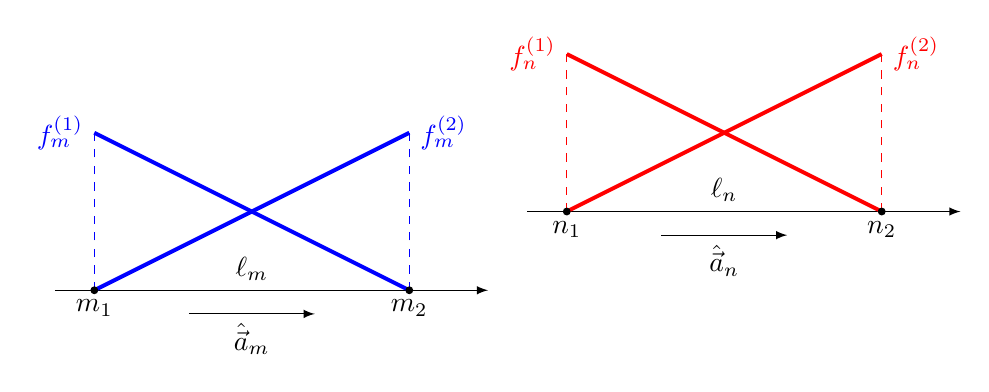
\begin{tikzpicture}[> = latex]
	\draw[->] (-0.5, 0) -- (5, 0);	
	
	\draw[blue, line width=0.5mm] (0, 2) node[left] {$f_m^{(1)}$} -- (4, 0);
	\draw[blue, line width=0.5mm] (0, 0) -- (4, 2) node[right] {$f_m^{(2)}$};
	
	\draw[blue, dashed] (0, 0) -- (0, 2);
	\draw[blue, dashed] (4, 0) -- (4, 2);
	\draw (0, 0) node[fill = black, circle, inner sep=0pt, minimum size = 1mm] {} node[below] {$m_1$};
	\draw (4, 0) node[fill = black, circle, inner sep=0pt, minimum size = 1mm] {} node[below] {$m_2$};
	
	\draw (2, 0) node[above] {$\ell_m$};
	
	\draw[->] (1.2, -0.3) -- node[below] {$\hat{\vec{a}}_m$} (2.8, -0.3);
	
	\draw[->] (5.5, 1) -- (11, 1);	
	
	\draw[red, line width=0.5mm] (6, 3) node[left] {$f_n^{(1)}$} -- (10, 1);
	\draw[red, line width=0.5mm] (6, 1) -- (10, 3) node[right] {$f_n^{(2)}$};
	\draw[red, dashed] (6, 1) -- (6, 3);
	\draw[red, dashed] (10, 1) -- (10, 3);
	\draw (6, 1) node[fill = black, circle, inner sep=0pt, minimum size = 1mm] {} node[below] {$n_1$};
	\draw (10, 1) node[fill = black, circle, inner sep=0pt, minimum size = 1mm] {} node[below] {$n_2$};
	
	\draw (8, 1) node[above] {$\ell_n$};
	
	\draw[->] (7.2, 0.7) -- node[below] {$\hat{\vec{a}}_n$} (8.8, 0.7);
\end{tikzpicture}